\documentclass[]{llncs} 
\usepackage{amsmath}
\usepackage{verbatim}
\usepackage{datatool}
\usepackage{tikz}
\usetikzlibrary{arrows,shapes}
\usepackage{graphics}

%\newtheorem{theorem}{Theorem}

\newcommand{\TODO}[1]{ {\color{red}{#1} }}
\newcommand{\com}[1]{ {\color{blue}{--- #1 ---}}}

\author{Valentin Mayer-Eichberger}

\institute{NICTA \\ University of New South Wales \\
\email{valentin.mayer-eichberger@nicta.com.au}}

\title{A SAT Encoding for the AtMostSeqCard Constraint}

\begin{document} \maketitle

\section{Introduction}

Give description of the car sequencing problem and the straight
forward encoding in IP/CNF. 

The naive CNF and IP encoding of the car sequencing benchmark is
far from optimal. In this paper we will show gradually how to come up
with a better encoding. 

\section{Motivation}

We are seeking an encoding that enforces GAC on the recently proposed
AtMostSeqCard constraint (\TODO{ref}). This constraint is not as expressive as the
Sequence constraint but is more suited for some benchmark problems and
has a linear filtering algorithm. Here we will show that there is a
compact CNF encoding that shows good results in the benchmark set of the
CSPLIB. Furthermore we will try to improve the bounds on the set of hard
instance. 

\section{Encoding of one AtMostSeqCard}

We will first show how to encode a cardinality constraint with a counter
encoding (\TODO{ref}) and then integrate the AtMostSeq by reusing the auxiliary
variables of the counter encoding. 

Over this whole section we will work with the following notation. Given
a set of consecutive positions $P=\{1\ldots n\}$ and a property that
holds at a position $i\in P$ iff the boolean variable $x_i$ is true. 

\subsection{Encoding of Counters}

We want to encode the following cardinality constraint

$$ \sum_{i\in \{1\ldots n\}} x_{i} = d $$

where $d$ is a fixed value.  We call the encoding for such a cardinality
constraint a counter encoding because we count exactly $d$ occurrences
over positions $\{1\ldots n\}$. 

We introduce the following variables: 

\begin{itemize}
    \item $y_{i,j}$ is true iff in the positions $1 \ldots i$ the
        property holds at least $j$ times.        
\end{itemize}

The following formula clarifies the relationship between $x$ and $y$.

$$ y_{i,j} \iff (j \leq \sum_{l=0}^{i} x_{l}) $$


\begin{figure}
\centering 
\caption{The variables $y_{i,j}$ with an upper bound $d$ of two over a
    sequence of 10. By preprocessing the variables corresponding to the
    cells containing $U$($L$) and above(below) are set to false (true).
    The question mark identifies unassigned variables of the counter
    encoding}
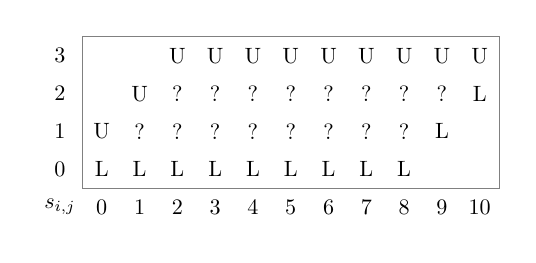
\begin{tikzpicture}[scale=0.8,every node/.style={scale=0.8}]
\node [matrix,ampersand replacement=\&,nodes={minimum size=6mm}]
%,nodes={fill=blue!20,minimum size=5mm}] 
    {
        \node {3}; \& \node (x) { }; \& \node { }; \& \node {U}; \& \node {U}; \& \node {U}; \& \node {U}; \& \node {U}; \& \node {U}; \& \node {U}; \& \node {U}; \& \node {U}; \\
        \node {2}; \& \node { }; \& \node {U}; \& \node {?}; \& \node {?}; \& \node {?}; \& \node {?}; \& \node {?}; \& \node {?}; \& \node {?}; \& \node {?}; \& \node {L}; \\
        \node {1}; \& \node {U}; \& \node {?}; \& \node {?}; \& \node {?}; \& \node {?}; \& \node {?}; \& \node {?}; \& \node {?}; \& \node {?}; \& \node {L}; \& \node { }; \\
        \node {0}; \& \node {L}; \& \node {L}; \& \node {L}; \& \node {L}; \& \node {L}; \& \node {L}; \& \node {L}; \& \node {L}; \& \node {L}; \& \node { }; \& \node (y) { }; \\
        \node {$s_{i,j}$}; \& \node {0}; \& \node {1}; \& \node {2}; \& \node {3}; \& \node {4}; \& \node {5}; \& \node {6}; \& \node {7}; \& \node {8}; \& \node {9}; \& \node {10}; \\
};
\draw[gray] (x.north west) rectangle (y.south east);
\end{tikzpicture}


\end{figure}

There are two types of binary clauses that relate the variables $y$ among
each other and two types of ternary clauses that coordinate $y$ with the
variables $x$.

\begin{equation}
    \bigwedge_{i \in \{0\ldots n-1\}} \bigwedge_{j \in\{0..d+1\}}
    \neg y_{i,j} \vee y_{i+1,j}
\end{equation}

\begin{equation}
    \bigwedge_{i \in \{1..n\}} \bigwedge_{j\in \{1..d+1\}}
    \neg y_{i,j} \vee y_{i-1,j-1}
\end{equation}

These clauses restrict the structure of the auxiliary variables to
consist of a counter. Now we need to relate these variables to $x$. 
First we restrict the counter not to increase if $x_{i}$ is
false. 


\begin{equation}
    \bigwedge_{i \in \{1\ldots n\}} \bigwedge_{j\in\{0..d+1\}}
    x_{i} \vee \neg y_{i,j} \vee y_{i-1,j}
\end{equation}

Second we define clauses that push  the counter up if $x_i$ is true. 

\begin{equation}
    \bigwedge_{i \in \{0\ldots n-1\}} \bigwedge_{j\in\{0..d\}}
    \neg x_{i} \vee \neg y_{i,j} \vee y_{i+1,j+1}
\end{equation}

Now we finally have to "initialize" the counter. 

\begin{equation}
y_{n,d} \wedge \left (\bigwedge_{i\in\{0\ldots n\}} y_{i,0} \right )\wedge \neg
    y_{0,1} \wedge \left(\bigwedge_{i\in\{0\ldots n\}} \neg
        y_{i,d+1}\right )
\end{equation}


\begin{figure}
\centering 
\caption{Taking the previous example and let $x_{i}$ be true for
    position 2 and 7. Then the resulting assignment to the counter
    variable is given in this table. }
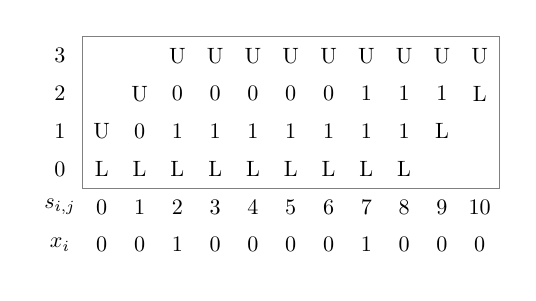
\begin{tikzpicture}[scale=0.8,every node/.style={scale=0.8}]    
\node [matrix,ampersand replacement=\&,nodes={minimum size=6mm}]
%,nodes={fill=blue!20,minimum size=5mm}] 
    {
        \node {3}; \& \node (x) { }; \& \node { }; \& \node {U}; \& \node {U}; \& \node {U}; \& \node {U}; \& \node {U}; \& \node {U}; \& \node {U}; \& \node {U}; \& \node {U}; \\
        \node {2}; \& \node { }; \& \node {U}; \& \node {0}; \& \node {0}; \& \node {0}; \& \node {0}; \& \node {0}; \& \node {1}; \& \node {1}; \& \node {1}; \& \node {L}; \\
        \node {1}; \& \node {U}; \& \node {0}; \& \node {1}; \& \node {1}; \& \node {1}; \& \node {1}; \& \node {1}; \& \node {1}; \& \node {1}; \& \node {L}; \& \node { }; \\
        \node {0}; \& \node {L}; \& \node {L}; \& \node {L}; \& \node {L}; \& \node {L}; \& \node {L}; \& \node {L}; \& \node {L}; \& \node {L}; \& \node { }; \& \node (y) { }; \\
        \node {$s_{i,j}$}; \& \node {0}; \& \node {1}; \& \node {2}; \& \node {3}; \& \node {4}; \& \node {5}; \& \node {6}; \& \node {7}; \& \node {8}; \& \node {9}; \& \node {10}; \\
        \node {$x_{i}$}; \& \node {0}; \& \node {0}; \& \node {1}; \& \node {0}; \& \node {0}; \& \node {0}; \& \node {0}; \& \node {1}; \& \node {0}; \& \node {0}; \& \node {0}; \\
};
\draw[gray] (x.north west) rectangle (y.south east);
\end{tikzpicture}


\end{figure}

It should be mentioned that with (6) we instruct the counter to measure
exactly $d$ occurences. It is easy to change the intializer to at most
$d$ or at least $d$ occurences. 

\subsection{Extending to AtMostSeqCard}

Given a sequence of boolean variables among exactly $d$ have to be true
and each window of size $q$ cannot contain more than $u$ true variables.
This is the AtMostSeqCard constraint: 

$$ \text{AtMostSeqCard}(u,q,d,[x_{1},\ldots,x_{n}]) \iff (\sum_{i=1}^n
x_{i} = d) \wedge \bigwedge_{i=1}^{n-q}(\sum_{l=1}^q x_{i+l} \leq u )$$

To archive GAC on this constraint we need to take the counter encoding
of the previous section and add the following binary clauses:

\begin{equation}
    \bigwedge_{\substack{i \in \{1 \ldots n\} \\ i-q \geq 0}}
    \bigwedge_{\substack{j\in\{1\ldots d+1\}\\ j-u \geq 0}}
    \neg y_{i,j} \vee y_{i-q,j-u}
\end{equation}               

This seems suprising! 

\begin{theorem}
    The clauses of counter encoding (1) to (5) with the clauses of (6)
    enforce GAC on the AtMostSeqCard for all partial assignment on
    variables $x_{i}$. 
\end{theorem}

We even have a stronger notion of propagation, because also on all
partial assignment on $y_{i,j}$ we archive GAC. 

\paragraph{Size of Encoding: } Let $s = n\cdot d-\text{upper and lower
triangle}$, then we generate $s$ auxiliary variables and $3\cdot s$
binary clauses and $2\cdot s$ tenery clauses. Size of a triange can be
computed by the hight $d$ and the slope $u/q$ and a little bit of
algebra, which leads to $d\cdot(u-q+\frac{d \cdot q}{u}) $. So the
number of variables $s$ should be

$$ s = d \cdot n - d \cdot(u-q+\frac{d \cdot q}{u}) $$

For example the at AtMostSeqCard$(u=4,q=8,d=12,n=22)$ would have 

$ 12\cdot 22- 12\cdot ( 4-8+\frac{12 \cdot 8}{4}) = 24$ variables, which
corresponds to the following example.  The power of the binary clauses
are best shown in the example taken from (\TODO{ref})

\begin{figure}
\centering 
\caption{Here we analyse the initial state of variables for a constraint
    with $u=4,q=8,d=12,n=22$. In this example we see that already
    $x_{7}$, $x_{8}$, $x_{15}$ and $x_{16}$ need to be set to false.
    Notice that for this particular case we only need 24 boolean
    variables to create the GAC encoding.}
\begin{tikzpicture}
\node [matrix,ampersand replacement=\&,nodes={minimum size=6mm}]
%,nodes={fill=blue!20,minimum size=5mm}] 
    {
\node{13}; \& \node (x) { }; \& \node { }; \& \node { }; \& \node { }; \& \node { }; \& \node { }; \& \node { }; \& \node { }; \& \node { }; \& \node { }; \& \node { }; \& \node { }; \& \node { }; \& \node { }; \& \node { }; \& \node { }; \& \node { }; \& \node { }; \& \node { }; \& \node { }; \& \node {U}; \& \node {U}; \& \node {U}; \\
\node{12}; \& \node { }; \& \node { }; \& \node { }; \& \node { }; \& \node { }; \& \node { }; \& \node { }; \& \node { }; \& \node { }; \& \node { }; \& \node { }; \& \node { }; \& \node { }; \& \node { }; \& \node { }; \& \node { }; \& \node { }; \& \node { }; \& \node { }; \& \node {U}; \& \node {?}; \& \node {?}; \& \node {L}; \\
\node{11}; \& \node { }; \& \node { }; \& \node { }; \& \node { }; \& \node { }; \& \node { }; \& \node { }; \& \node { }; \& \node { }; \& \node { }; \& \node { }; \& \node { }; \& \node { }; \& \node { }; \& \node { }; \& \node { }; \& \node { }; \& \node { }; \& \node {U}; \& \node {?}; \& \node {?}; \& \node {L}; \& \node { }; \\
\node{10}; \& \node { }; \& \node { }; \& \node { }; \& \node { }; \& \node { }; \& \node { }; \& \node { }; \& \node { }; \& \node { }; \& \node { }; \& \node { }; \& \node { }; \& \node { }; \& \node { }; \& \node { }; \& \node { }; \& \node { }; \& \node {U}; \& \node {?}; \& \node {?}; \& \node {L}; \& \node { }; \& \node { }; \\
\node{9}; \& \node { }; \& \node { }; \& \node { }; \& \node { }; \& \node { }; \& \node { }; \& \node { }; \& \node { }; \& \node { }; \& \node { }; \& \node { }; \& \node { }; \& \node {U}; \& \node {U}; \& \node {U}; \& \node {U}; \& \node {U}; \& \node {?}; \& \node {?}; \& \node {L}; \& \node { }; \& \node { }; \& \node { }; \\
\node{8}; \& \node { }; \& \node { }; \& \node { }; \& \node { }; \& \node { }; \& \node { }; \& \node { }; \& \node { }; \& \node { }; \& \node { }; \& \node { }; \& \node {U}; \& \node {?}; \& \node {?}; \& \node {L}; \& \node {L}; \& \node {L}; \& \node {L}; \& \node {L}; \& \node { }; \& \node { }; \& \node { }; \& \node { }; \\
\node{7}; \& \node { }; \& \node { }; \& \node { }; \& \node { }; \& \node { }; \& \node { }; \& \node { }; \& \node { }; \& \node { }; \& \node { }; \& \node {U}; \& \node {?}; \& \node {?}; \& \node {L}; \& \node { }; \& \node { }; \& \node { }; \& \node { }; \& \node { }; \& \node { }; \& \node { }; \& \node { }; \& \node { }; \\
\node{6}; \& \node { }; \& \node { }; \& \node { }; \& \node { }; \& \node { }; \& \node { }; \& \node { }; \& \node { }; \& \node { }; \& \node {U}; \& \node {?}; \& \node {?}; \& \node {L}; \& \node { }; \& \node { }; \& \node { }; \& \node { }; \& \node { }; \& \node { }; \& \node { }; \& \node { }; \& \node { }; \& \node { }; \\
\node{5}; \& \node { }; \& \node { }; \& \node { }; \& \node { }; \& \node {U}; \& \node {U}; \& \node {U}; \& \node {U}; \& \node {U}; \& \node {?}; \& \node {?}; \& \node {L}; \& \node { }; \& \node { }; \& \node { }; \& \node { }; \& \node { }; \& \node { }; \& \node { }; \& \node { }; \& \node { }; \& \node { }; \& \node { }; \\
\node{4}; \& \node { }; \& \node { }; \& \node { }; \& \node {U}; \& \node {?}; \& \node {?}; \& \node {L}; \& \node {L}; \& \node {L}; \& \node {L}; \& \node {L}; \& \node { }; \& \node { }; \& \node { }; \& \node { }; \& \node { }; \& \node { }; \& \node { }; \& \node { }; \& \node { }; \& \node { }; \& \node { }; \& \node { }; \\
\node{3}; \& \node { }; \& \node { }; \& \node {U}; \& \node {?}; \& \node {?}; \& \node {L}; \& \node { }; \& \node { }; \& \node { }; \& \node { }; \& \node { }; \& \node { }; \& \node { }; \& \node { }; \& \node { }; \& \node { }; \& \node { }; \& \node { }; \& \node { }; \& \node { }; \& \node { }; \& \node { }; \& \node { }; \\
\node{2}; \& \node { }; \& \node {U}; \& \node {?}; \& \node {?}; \& \node {L}; \& \node { }; \& \node { }; \& \node { }; \& \node { }; \& \node { }; \& \node { }; \& \node { }; \& \node { }; \& \node { }; \& \node { }; \& \node { }; \& \node { }; \& \node { }; \& \node { }; \& \node { }; \& \node { }; \& \node { }; \& \node { }; \\
\node{1}; \& \node {U}; \& \node {?}; \& \node {?}; \& \node {L}; \& \node { }; \& \node { }; \& \node { }; \& \node { }; \& \node { }; \& \node { }; \& \node { }; \& \node { }; \& \node { }; \& \node { }; \& \node { }; \& \node { }; \& \node { }; \& \node { }; \& \node { }; \& \node { }; \& \node { }; \& \node { }; \& \node { }; \\
\node{0}; \& \node {L}; \& \node {L}; \& \node {L}; \& \node { }; \& \node { }; \& \node { }; \& \node { }; \& \node { }; \& \node { }; \& \node { }; \& \node { }; \& \node { }; \& \node { }; \& \node { }; \& \node { }; \& \node { }; \& \node { }; \& \node { }; \& \node { }; \& \node { }; \& \node { }; \& \node { }; \& \node (y) { }; \\
\node{j/i}; \& \node {0}; \& \node {1}; \& \node {2}; \& \node {3}; \& \node {4}; \& \node {5}; \& \node {6}; \& \node {7}; \& \node {8}; \& \node {9}; \& \node {10}; \& \node {11}; \& \node {12}; \& \node {13}; \& \node {14}; \& \node {15}; \& \node {16}; \& \node {17}; \& \node {18}; \& \node {19}; \& \node {20}; \& \node {21}; \& \node {22}; \\
\node{$x_i$}; \& \node { }; \& \node { }; \& \node { }; \& \node { }; \&
        \node { }; \& \node { }; \& \node { }; \& \node {\textbf{0}}; \&
        \node {\textbf{0}}; \& \node { }; \& \node { }; \& \node { }; \&
        \node { }; \& \node { }; \& \node { }; \& \node {\textbf{0}}; \&
        \node {\textbf{0}}; \& \node { }; \& \node { }; \& \node { }; \& \node { }; \& \node { }; \& \node { }; \\
};
\draw[gray] (x.north west) rectangle (y.south east);
\end{tikzpicture}


\end{figure}

\begin{figure}
\centering 
\caption{State of the auxiliary variables for $u=4,q=8,d=12,n=22$ and
    choices $x_{1}$ and $x_{13}$ to true and $x_{12}$, $x_{14}$ and
    $x_{21}$ to false. Notice the amount of propagation due to the
    clauses of the AtMostSeqCard constraint, also notice that variable
$x_{1}$ was a redundant choice. Normal font= choice, bold = propagated,
()= earlier propagated, green arrow positve implication, red arrow
negative implication by (6).}
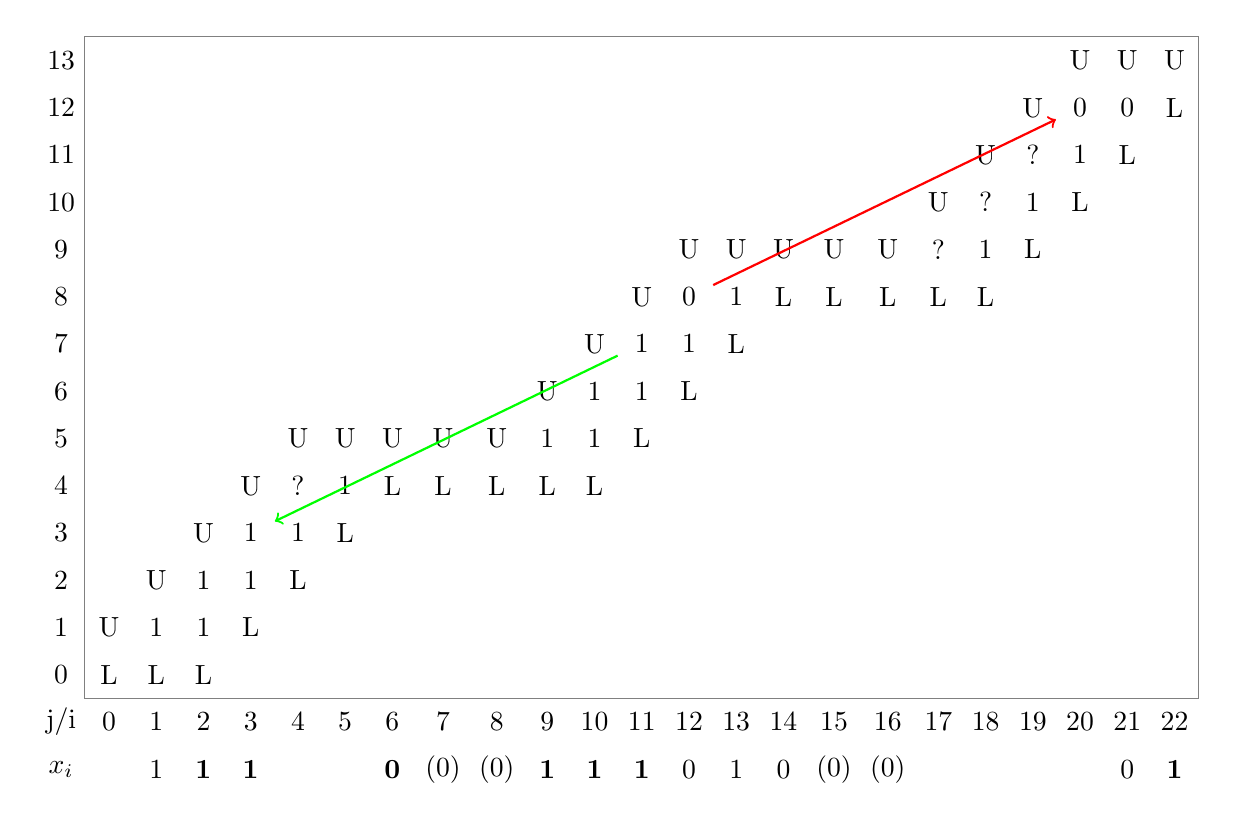
\begin{tikzpicture}
\node [matrix,ampersand replacement=\&,nodes={minimum size=6mm}]
    {
\node {13}; \& \node (x) { }; \& \node { }; \& \node { }; \& \node { }; \& \node { }; \& \node { }; \& \node { }; \& \node { }; \& \node { }; \& \node { }; \& \node { }; \& \node { }; \& \node { }; \& \node { }; \& \node { }; \& \node { }; \& \node { }; \& \node { }; \& \node { }; \& \node { }; \& \node {U}; \& \node {U}; \& \node {U}; \\
\node {12}; \& \node { }; \& \node { }; \& \node { }; \& \node { }; \&
        \node { }; \& \node { }; \& \node { }; \& \node { }; \& \node {
    }; \& \node { }; \& \node { }; \& \node { }; \& \node { }; \& \node
        { }; \& \node { }; \& \node { }; \& \node { }; \& \node { }; \&
        \node { }; \& \node {U}; \& \node (b) {0}; \& \node {0}; \& \node {L}; \\
\node {11}; \& \node { }; \& \node { }; \& \node { }; \& \node { }; \& \node { }; \& \node { }; \& \node { }; \& \node { }; \& \node { }; \& \node { }; \& \node { }; \& \node { }; \& \node { }; \& \node { }; \& \node { }; \& \node { }; \& \node { }; \& \node { }; \& \node {U}; \& \node {?}; \& \node {1}; \& \node {L}; \& \node { }; \\
\node {10}; \& \node { }; \& \node { }; \& \node { }; \& \node { }; \& \node { }; \& \node { }; \& \node { }; \& \node { }; \& \node { }; \& \node { }; \& \node { }; \& \node { }; \& \node { }; \& \node { }; \& \node { }; \& \node { }; \& \node { }; \& \node {U}; \& \node {?}; \& \node {1}; \& \node {L}; \& \node { }; \& \node { }; \\
\node {9}; \& \node { }; \& \node { }; \& \node { }; \& \node { }; \& \node { }; \& \node { }; \& \node { }; \& \node { }; \& \node { }; \& \node { }; \& \node { }; \& \node { }; \& \node {U}; \& \node {U}; \& \node {U}; \& \node {U}; \& \node {U}; \& \node {?}; \& \node {1}; \& \node {L}; \& \node { }; \& \node { }; \& \node { }; \\
\node {8}; \& \node { }; \& \node { }; \& \node { }; \& \node { }; \& \node { }; \& \node { }; \& \node { }; \& \node { }; \& \node { }; \& \node { }; \& \node { }; \& \node {U}; \& \node (a) {0}; \& \node {1}; \& \node {L}; \& \node {L}; \& \node {L}; \& \node {L}; \& \node {L}; \& \node { }; \& \node { }; \& \node { }; \& \node { }; \\
\node {7}; \& \node { }; \& \node { }; \& \node { }; \& \node { }; \&
        \node { }; \& \node { }; \& \node { }; \& \node { }; \& \node {
    }; \& \node { }; \& \node {U}; \& \node (c) {1}; \& \node {1}; \& \node {L}; \& \node { }; \& \node { }; \& \node { }; \& \node { }; \& \node { }; \& \node { }; \& \node { }; \& \node { }; \& \node { }; \\
\node {6}; \& \node { }; \& \node { }; \& \node { }; \& \node { }; \& \node { }; \& \node { }; \& \node { }; \& \node { }; \& \node { }; \& \node {U}; \& \node {1}; \& \node {1}; \& \node {L}; \& \node { }; \& \node { }; \& \node { }; \& \node { }; \& \node { }; \& \node { }; \& \node { }; \& \node { }; \& \node { }; \& \node { }; \\
\node {5}; \& \node { }; \& \node { }; \& \node { }; \& \node { }; \& \node {U}; \& \node {U}; \& \node {U}; \& \node {U}; \& \node {U}; \& \node {1}; \& \node {1}; \& \node {L}; \& \node { }; \& \node { }; \& \node { }; \& \node { }; \& \node { }; \& \node { }; \& \node { }; \& \node { }; \& \node { }; \& \node { }; \& \node { }; \\
\node {4}; \& \node { }; \& \node { }; \& \node { }; \& \node {U}; \& \node {?}; \& \node {1}; \& \node {L}; \& \node {L}; \& \node {L}; \& \node {L}; \& \node {L}; \& \node { }; \& \node { }; \& \node { }; \& \node { }; \& \node { }; \& \node { }; \& \node { }; \& \node { }; \& \node { }; \& \node { }; \& \node { }; \& \node { }; \\
        \node {3}; \& \node { }; \& \node { }; \& \node {U}; \& \node
        (d) {1}; \& \node {1}; \& \node {L}; \& \node { }; \& \node { }; \& \node { }; \& \node { }; \& \node { }; \& \node { }; \& \node { }; \& \node { }; \& \node { }; \& \node { }; \& \node { }; \& \node { }; \& \node { }; \& \node { }; \& \node { }; \& \node { }; \& \node { }; \\
\node {2}; \& \node { }; \& \node {U}; \& \node {1}; \& \node {1}; \& \node {L}; \& \node { }; \& \node { }; \& \node { }; \& \node { }; \& \node { }; \& \node { }; \& \node { }; \& \node { }; \& \node { }; \& \node { }; \& \node { }; \& \node { }; \& \node { }; \& \node { }; \& \node { }; \& \node { }; \& \node { }; \& \node { }; \\
\node {1}; \& \node {U}; \& \node {1}; \& \node {1}; \& \node {L}; \& \node { }; \& \node { }; \& \node { }; \& \node { }; \& \node { }; \& \node { }; \& \node { }; \& \node { }; \& \node { }; \& \node { }; \& \node { }; \& \node { }; \& \node { }; \& \node { }; \& \node { }; \& \node { }; \& \node { }; \& \node { }; \& \node { }; \\
\node {0}; \& \node {L}; \& \node {L}; \& \node {L}; \& \node { }; \& \node { }; \& \node { }; \& \node { }; \& \node { }; \& \node { }; \& \node { }; \& \node { }; \& \node { }; \& \node { }; \& \node { }; \& \node { }; \& \node { }; \& \node { }; \& \node { }; \& \node { }; \& \node { }; \& \node { }; \& \node { }; \& \node (y) { }; \\
\node {j/i}; \& \node {0}; \& \node {1}; \& \node {2}; \& \node {3}; \& \node {4}; \& \node {5}; \& \node {6}; \& \node {7}; \& \node {8}; \& \node {9}; \& \node {10}; \& \node {11}; \& \node {12}; \& \node {13}; \& \node {14}; \& \node {15}; \& \node {16}; \& \node {17}; \& \node {18}; \& \node {19}; \& \node {20}; \& \node {21}; \& \node {22}; \\
        \node{$x_i$}; \& \node {}; \& \node {1}; \& \node {\textbf{1}}; \& \node { \textbf{1}}; \& \node { }; \& \node { }; \& \node {\textbf{0} }; \& \node {(0)}; \& \node {(0)}; \& \node {\textbf{1} }; \& \node {\textbf{1} }; \& \node {\textbf{1} }; \& \node {0}; \& \node {1}; \& \node {0}; \& \node {(0)}; \& \node {(0)}; \& \node { }; \& \node { }; \& \node { }; \& \node { }; \& \node {0}; \& \node {\textbf{1}}; \\
};
\draw[thick,red,->, sloped, above] (a) -- (b); 
\draw[thick,green,->,bend right] (c) -- (d); 
\draw[gray] (x.north west) rectangle (y.south east);
\end{tikzpicture}       

\end{figure}

\section{Encoding of Carsequencing}

We need to relate the cars and options as in the problem specification.
This can be done in two ways. First the straight forward way. 

\subsection{Relating Cars and Option directly}

Let $C$ be the index set identifying a class and $O$ be the index set
for options. The instance for a car sequencing problem is given by a
mapping $m : C\rightarrow 2^O$, relating to each class a set of options.
For each class we have a cardinality constraint and for each option a
AtMostSeq constraint. From this we can construct for each option and for
each class a AtMostSeqCard constraint (since all cars have to be
assigend). 

Each such AtMostSeqCard constraint is encoded into SAT. In addition we
need to relate classes and options on each position. This is done by the
following clauses.  Let $m':O \rightarrow 2^C$ be the mapping relating
to each option the corresponding classes. 

\begin{equation}
    \bigwedge_{i\in \{1\ldots n\}} \bigwedge_{\substack{c \in C \\ o \in m(c)}} \neg x_{i,c} \vee x_{i,o}
\end{equation}

and the reverse

\begin{equation}
    \bigwedge_{i \in \{1\dots n\}} \bigwedge_{o\in O} \left(\neg x_{i,o} \vee
    \bigvee_{c \in m'(o)} x_{i,c}\right)
\end{equation}

Notice in an ASP encoding this would be modelled by one rule and the
completion semantics covers for the reverse case. 

\subsection{The Purist's Way}

Here we will show that there is an encoding of the car sequencing
problem that does not use at all the variables $x_{i,k}$. The encoding
builds entirely on the auxiliary variables $y_{i,j,k}$ and their
relationship. This is rather surprising. Here the idea: 

For each position in the sequence, the
sum of true $y$ for all cars that have option $o$ need to be the same
size as the number of true $y$ for $o$. As a formula, for all positions
$i$ and options $ o \in O$ it has to hold: 

$$ \sum_{j} y_{i,j,o} = \sum_{c \in m'(o)} \sum_j y_{i,j,c} $$

Encoding this restriction (e.g. by a counter!) should be enough to fully
grasp the car sequencing problem. However, the size of this encoding
is considerable bigger  and it will have a different type of propagation, as
it cannot branch on putting cars or options in positions. 


\section{Evaluation}

Best of results that can be robustly (standard heuristics) archived by
current sat solvers. I compared newest version of minisat, lingeling,
cryptominisat, glucose and clasp and they all consistently find
solutions within 1h runtime. 

\DTLsetseparator{,}
\DTLloaddb[keys={res,set1,set2,set3,set4}]{all}{table1.csv}

\begin{table}[htbp]
    \caption{}
    \centering
    \DTLdisplaydb{all}
\end{table}


This is by far better than most papers evaluating the car sequencing
problem on some specialized algorithm (e.g. branch and bound) or special
constraint (CP) or optimization (IP). 

For the set 4 a more detailed view is interesting as the benchmark
targets the optimization version of the car sequencing problem. 

\DTLsetseparator{,}
\DTLloaddb[keys={name,min,max,LING,sec}]{set4}{table2.csv}

\begin{table}[htbp]
    \caption{Solutions to the benchmark proposed in \TODO{ref} with
    lower and upper bounds on the target function (min,max) and this
compared to solutions on the decision version  SAT encoding with lingeling (LING). }
    \centering
    \DTLdisplaydb{set4}
\end{table}


We can solve all 7 satisfiable instances and prove 13/23 instances to be
unsatisfiable. 


\section{Extensions}

\begin{itemize}
    \item Optimizations: there are two definitions of the cost function
        for the car sequencing problem. First is to allow arbitrary cars
        without any options and minimize the number of cars with
        options. And second is to minimize the number of windows that
        exceed the capacity constraint on their options. It would be
        interesting to compare both definition and to evaluate against
        published results in the literature. There are still gaps
        between known upper and lower bounds. 
    \item There is a natural extension of the AtMostSeqCard constraint
        that to a cyclic version and in the same and natural way we can
        extend the encoding given above. It would be interesting to find
        good benchmarks. 
    \item The Sequence constraint consists of a sequence of among
        constraints and we should compare this encoding to the known CNF
        encodings and filtering algorithms in the literature. 
\end{itemize}




\end{document}
